% !TeX spellcheck = cs_CZ
%---------------------------------------------------------------------------------------------------
% mai2ch04.tex
%---------------------------------------------------------------------------------------------------
\chapter{Obyčejné diferenciální rovnice}\label{mai:IIchapIV}
\minitoc
  \section{Diferenciální rovnice 1. řádu}
    Řada fyzikálních principů má tvar výroku, resp. vztahu mezi jistými veličinami (funkcemi) a
    jejich změnami, vztaženými ke zvoleným nezávisle proměnným pa\-ra\-me\-trům (čas, souřadnice).
    Změny (okamžité, lokální) se nejlépe vystihují pomocí derivací. Takový zákon má pak charakter
    vztahu mezi uvažovanými veličinami a jejich derivacemi. Nejčastěji bývá vztah vyjádřen formou
    rovnosti:
    \begin{itemize}
   	  \item Newtonůw zákon: okamžitá změna hybnosti $p(t) = m(t)\cdot v(t)$ pohybujícího se
         	objektu je úměrná působící síle $F(t)$ v každém okamžiku $t$ zvoleného časového rozmezí
        	$$\frac{d}{dt}\left(m(t)\cdot v(t)\right) = F(t)\quad t\in\langle\alpha, \beta\rangle$$
      \item Kirchhoffův zákon pro LR – obvod: v okamžiku $t$ je součet napětí na cívce s indukčnosti
            $L$ a na rezistoru o odporu $R$ roven napětí $U(t)$ na svorkách zdroje. Tuto rovnost pak
            zapisujeme ve tvaru (pro L,R = konst)
            \begin{equation}
              L\frac{di(t)}{dt}+Ri=u(t), 
            \end{equation}
            kde $i=i(t)\ldots$ funkce popisující závislost proudu na čase.
    \end{itemize}
    
    Chceme-li určit funkci $i=i(t)$ popisující průběh proudu v obvodu tak, aby byl splněn příslušný
    K.z. a současně, aby byl splněn požadavek na počáteční stav:
    \begin{equation}
        L\frac{di(t)}{dt}+Ri(t)=U,\quad i(0)=I_0,\quad t\in\langle 0,+\infty)
    \end{equation}
    Metodami uvedenými později stanovíme právě jednu funkci $i=i(t)$, která je řešením dané tzv.
    \textbf{počáteční úlohy}.
    \begin{equation}
      \begin{array}{c}
         i(t)=I_0\left(1-e^{-\frac{R}{L}t}\right),\quad t\in\langle 0,+\infty), \\
         lim_{t\rightarrow +\infty}i(t)=\frac{U_0}{R},\quad lim_{t\rightarrow +0}i(t)=I_0=i(0)
      \end{array}
    \end{equation}
    \begin{itemize}
      \item tedy obvykle formulujeme úlohu najít jistou funkci tak, aby zákon byl splněn tj.
            Kirchhoffův zákon užijeme k tomu, abychom nalezli funkci $i(t)$
      \item užijeme-li rovnosti vyjadřující takový zákon k tomu, abychom určili funkci, která v
            takovém vztahu vystupuje spolu s derivacemi, stává se tento požadavek úlohou, která má
            charakter rovnice s derivacemi, neboli diferenciální rovnice. Funkce, která požadavek
            splňuje, se pak nazývá řešení diferenciální rovnice.
    \end{itemize}
    
    \begin{figure}
      \centering
      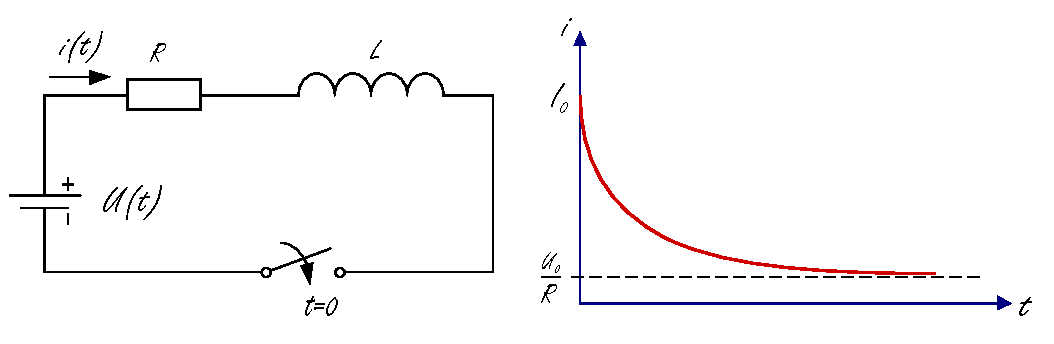
\includegraphics[width=\linewidth]{mai_fig032.pdf}
      \caption{Graf průběhu proudu $i(t)$ po sepnutí spínače v době $t=0$.}
      \label{mai:fig032}
    \end{figure}
%---------------------------------------------------------------------------------------------------
\printbibliography[title={Seznam literatury}, heading=subbibliography]
\addcontentsline{toc}{section}{Seznam literatury}